\documentclass[border=10pt,multi,tikz]{standalone}
\usepackage{tikz}
\usetikzlibrary{mindmap}
\pagestyle{empty}
\begin{document}
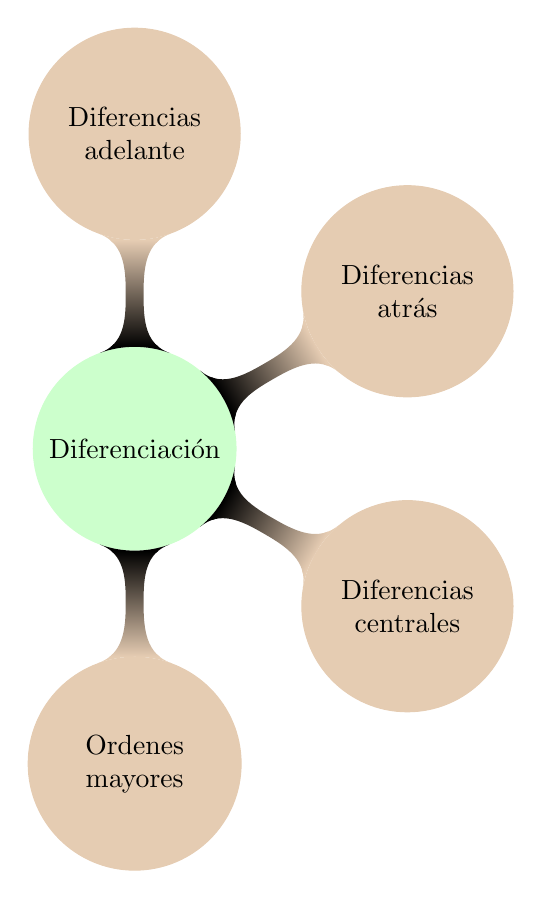
\begin{tikzpicture}[grow cyclic, text width=2.3cm, align=flush center, every node/.style={concept}, concept color=brown!40, 
    level 1/.style={level distance=4cm,sibling angle=60}]
    \node[concept color=green!20, level distance=5cm] {Diferenciación} [clockwise from=90]
        child { node {Diferencias adelante}}
        child { node {Diferencias atrás}}
        child { node {Diferencias centrales}}
        child { node {Ordenes mayores}}
;
\end{tikzpicture}
\end{document}